Según la nota de aplicación de Linear Technology~\cite{Zhang2015}, la transferencia de $\hat{d}$ a $\hat{v}_o$ para un convertidor \textit{buck} es
\[
    G_{dv}(s) = \frac{\hat{v}_o}{\hat{d}} = V_{IN} \cdot \frac{1 + s/\omega_{z\text{-ESR}}}{1 + \dfrac{s}{Q\omega_0} + \dfrac{s^2}{\omega_0^2}} \, ,
\]
donde los parámetros de la planta son
\begin{align*}
    \omega_{z\text{-ESR}} &= \frac{1}{r_C \cdot C} \, , \\[6pt]
    \omega_0 &= 2\pi f_0 = \frac{1}{\sqrt{L \cdot C}} \cdot \sqrt{\frac{1 + r_L/R}{1 + r_C/R}} \;\approx\; \frac{1}{\sqrt{L \cdot C}} \, , \\[6pt]
    Q &= \frac{1}{\omega_0} \cdot \frac{1}{\dfrac{L}{r_L + R} + C\left(r_C + r_L \!\parallel\! R\right)} \;\approx\; \sqrt{L \cdot C} \cdot \frac{1}{\dfrac{L}{R} + C(r_C + r_L)} \, .
\end{align*}
La linealización es válida si $r_L \ll R$ y $r_C \ll R$, condición que se cumple en el diseño dado que la carga mínima es de $6\,\Omega$ ($9{.}3\,\text{V}/1{.}6\,\text{A} \approx 5{.}8\,\Omega$). En resumen, el sistema tiene un cero real ($\omega_{z\text{-ESR}}$) y un par de polos complejos conjugados de resonancia ($\omega_0$, $Q$). Notar que esto es una linealización alrededor de un punto de equilibrio usando un modelo promediado.

\begin{figure}[H]
    \centering
    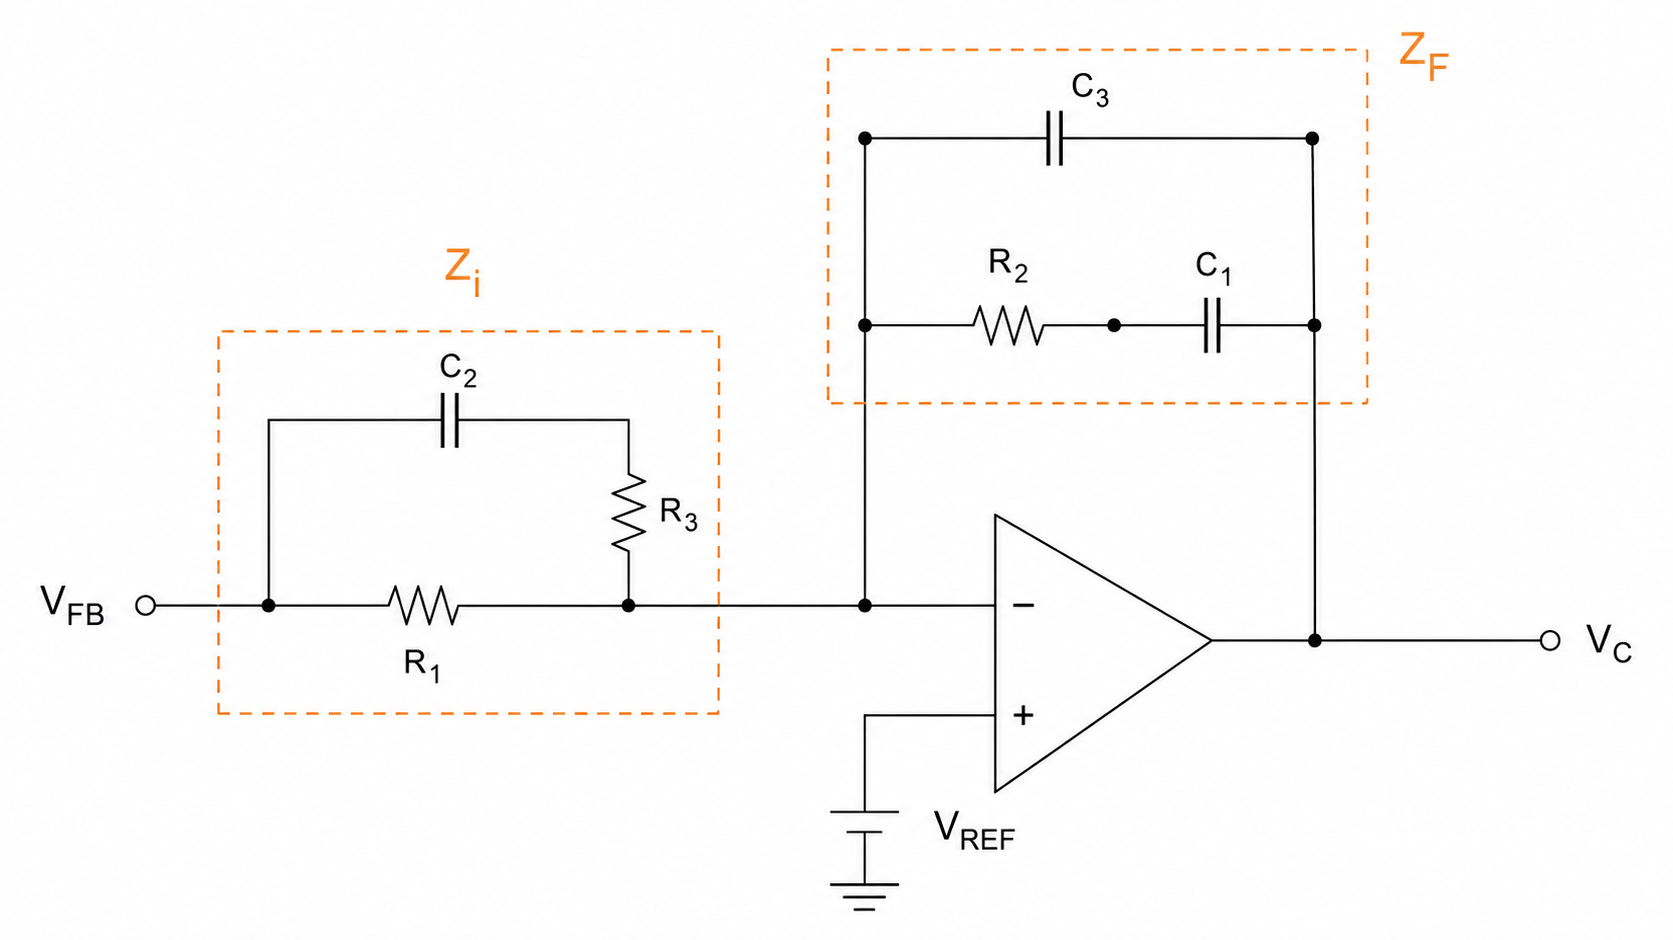
\includegraphics[width = 0.8\textwidth]{img/red_compensacion.png}
    \caption{Red de compensación tipo III.}
    \label{fig:red_compensacion}
\end{figure}

Se propone una red de compensación tipo III (véase la Figura~\ref{fig:red_compensacion}). Llamando $Z_i$ y $Z_f$ a la impedancia de entrada y de retroalimentación respectivamente se tiene
\[
    A(s) = \frac{V_c(s)}{V_{FB}(s)} = -\frac{Z_f}{Z_i}
\]
con
\[
    Z_i = R_1 \,\Big\|\, \left(R_3 + \frac{1}{C_2 s}\right) \quad \text{y} \quad
    Z_f = \frac{1}{C_3 s} \,\Big\|\, \left(R_2 + \frac{1}{C_1 s}\right) \, .
\]

Recordando que $R + \dfrac{1}{Cs} = \dfrac{RCs + 1}{Cs} = R \cdot \dfrac{s + 1/RC}{s}$, la función de transferencia del compensador resulta ser un integrador con 2 polos y 2 ceros:
\[
    A(s) = -\frac{\omega_1}{s} \cdot \frac{\left(1 + s/\omega_{z_1}\right)\left(1 + s/\omega_{z_2}\right)}{\left(1 + s/\omega_{p_1}\right)\left(1 + s/\omega_{p_2}\right)} \, ,
\]
donde los ceros, polos y ganancia del integrador quedan determinados por los componentes según
\begin{align}
    \omega_1    &= \frac{1}{R_1(C_1 + C_3)}\,;  \label{eq:w1} \\[4pt]
    \omega_{z_1} &= \frac{1}{R_2 C_1}          \quad \text{(cero de $Z_f$, cuando $Z_f \to 0$)}\,; \label{eq:wz1} \\[4pt]
    \omega_{z_2} &= \frac{1}{(R_1 + R_3)C_2}   \quad \text{(cero de $Z_i$, cuando $Z_i \to \infty$)}\,; \label{eq:wz2} \\[4pt]
    \omega_{p_1} &= \frac{1}{R_3 C_2}           \quad \text{(polo de $Z_i$, cuando $Z_i \to 0$)}\,; \label{eq:wp1} \\[4pt]
    \omega_{p_2} &= \frac{1}{R_2 \,\dfrac{C_1 C_3}{C_1 + C_3}} \quad \text{(polo de $Z_f$, cuando $Z_f \to 0$)}\,; \label{eq:wp2}
\end{align}
siendo $\omega_1$ la frecuencia a la cual la ganancia del integrador llega a $0\,\text{dB}$ (frecuencia de cruce o ancho de banda).

La observación clave es que por la construcción del modulador PWM, $V_c$ debe encontrarse entre $4\,\text{V}$ y $5\,\text{V}$. La relación entre el \textit{duty cycle} y la tensión de control es lineal:
\[
    d = \frac{V_c - 4\,\text{V}}{5\,\text{V} - 4\,\text{V}} \, ,
\]
por lo que $\hat{d} \approx \hat{v}_c$ y la transferencia del compensador referida a $\hat{v}_o$ es
\[
    \frac{\hat{v}_c}{\hat{v}_o}(s) = -\frac{\omega_1}{s} \cdot \frac{\left(1 + s/\omega_{z_1}\right)\left(1 + s/\omega_{z_2}\right)}{\left(1 + s/\omega_{p_1}\right)\left(1 + s/\omega_{p_2}\right)} \,.
\]

Las restricciones de diseño que impone la estrategia de cancelación son las siguientes.

\begin{enumerate}
    \item \textbf{Cancelación del polo doble de resonancia} ($\omega_{z_1} = \omega_{z_2} = \omega_0$).
    \[
        \frac{1}{R_2 C_1} = \frac{1}{(R_1 + R_3)C_2} = \frac{1}{\sqrt{LC}}
    \]

    \item \textbf{Cancelación del cero de la ESR} ($\omega_{p_1} = \omega_{z\text{-ESR}}$).
    \[
        \frac{1}{R_3 C_2} = \frac{1}{r_C \cdot C}
    \]

    \item \textbf{Filtrado del ruido de conmutación} ($\omega_{p_2} = 2\pi f_{sw}/k$, con $k = 10$).
    \[
        \frac{1}{R_2 \,\dfrac{C_1 C_3}{C_1 + C_3}} = \frac{2\pi f_{sw}}{10} \approx 82\,000\,\text{rad/s}
    \]
\end{enumerate}

Se tienen 5 restricciones y 6 incógnitas ($R_1, R_2, R_3, C_1, C_2, C_3$), por lo que el sistema tiene \textbf{1 grado de libertad}. Aplicando logaritmo a cada una de las relaciones~\eqref{eq:w1}--\eqref{eq:wp2}, el sistema se vuelve lineal en las variables $x_i = \ln(\cdot)$. Definiendo
\[
    \mathbf{x} = \begin{bmatrix} \ln R_1 \\ \ln R_2 \\ \ln R_3 \\ \ln C_1 \\ \ln C_2 \\ \ln C_3 \end{bmatrix} \quad \text{e} \quad
    \mathbf{y} = \begin{bmatrix} \ln \omega_1 \\ \ln \omega_{z_1} \\ \ln \omega_{z_2} \\ \ln \omega_{p_1} \\ \ln \omega_{p_2} \end{bmatrix}
\]
el sistema $\mathbf{y} = A\,\mathbf{x}$ tiene la siguiente forma (bajo la aproximación $R_1 \gg R_3$, $C_1 \gg C_3$).

\begin{equation*}
    \begin{pmatrix} \ln \omega_1 \\ \ln \omega_{z_1} \\ \ln \omega_{z_2} \\ \ln \omega_{p_1} \\ \ln \omega_{p_2} \end{pmatrix}
    =
    \begin{pmatrix}
        -1 & 0  & 0  & -1 & 0  & 0  \\
         0 & -1 & 0  & -1 & 0  & 0  \\
        -1 & 0  & 0  & 0  & -1 & 0  \\
         0 & 0  & -1 & 0  & -1 & 0  \\
         0 & -1 & 0  & 0  & 0  & -1
    \end{pmatrix}
    \begin{pmatrix} \ln R_1 \\ \ln R_2 \\ \ln R_3 \\ \ln C_1 \\ \ln C_2 \\ \ln C_3 \end{pmatrix}
\end{equation*}

Se puede verificar que el núcleo de $A$ está generado por
\[
    \mathbf{N}_0 = \begin{pmatrix} 1 \\ 1 \\ 1 \\ -1 \\ -1 \\ -1 \end{pmatrix}
    \qquad \text{ya que} \qquad A\,\mathbf{N}_0 = \mathbf{0} \,.\quad \checkmark
\]

Por lo tanto, el conjunto de soluciones forma una recta: si $\mathbf{x}_0$ es solución, entonces $\mathbf{x}_0 + \alpha\,\mathbf{N}_0$ también lo es para todo $\alpha \in \mathbb{R}$.

Para evitar trabajar con valores numéricos muy extremos, se expresan las resistencias en k$\Omega$ y los capacitores en nF. En ese caso, $RC = R[\text{k}\Omega] \cdot 10^3 \cdot C[\text{nF}] \cdot 10^{-9} = \frac{R[\text{k}\Omega]\,C[\text{nF}]}{10^6}$, con lo que
\[
    \omega = \frac{10^6}{R[\text{k}\Omega]\,C[\text{nF}]}
\]
y el sistema lineal logarítmico resulta
\begin{align*}
    \ln \omega_1    - \ln(10^6) &= -\ln R_1 - \ln C_1\,; \\
    \ln \omega_{z_1} - \ln(10^6) &= -\ln R_2 - \ln C_1\,; \\
    \ln \omega_{z_2} - \ln(10^6) &= -\ln R_1 - \ln C_2\,; \\
    \ln \omega_{p_1} - \ln(10^6) &= -\ln R_3 - \ln C_2\,; \\
    \ln \omega_{p_2} - \ln(10^6) &= -\ln R_2 - \ln C_3\,.
\end{align*}
Solo cambia el vector $\mathbf{y}$ (se le resta $\ln(10^6)$ a cada componente); la matriz $A$ permanece idéntica.

Sea $\mathbf{x}_0 = \operatorname*{arg\,min}_{\mathbf{x}} \|\mathbf{y} - A\mathbf{x}\|^2$ la solución de mínimos cuadrados al sistema simplificado ($R_1 \gg R_3$, $C_1 \gg C_3$). La familia de soluciones es
\begin{equation*}
    \mathbf{x}_0 + \alpha\,\mathbf{N}_0 = \ln \begin{pmatrix} R_1 \\ R_2 \\ R_3 \\ C_1 \\ C_2 \\ C_3 \end{pmatrix} + \alpha \begin{pmatrix} 1 \\ 1 \\ 1 \\ -1 \\ -1 \\ -1 \end{pmatrix}
    \quad \Rightarrow \quad \ln R_1 + \alpha = \ln(\alpha' R_1) \quad \text{con } \alpha' = e^\alpha \, .
\end{equation*}
Es decir, barrer $\alpha$ equivale a escalar todas las resistencias por $\alpha'$ y todos los capacitores por $1/\alpha'$, con $0{,}1 < \alpha' < 10$ ($\ln 0{,}1 < \alpha < \ln 10$). Barriendo a lo largo de esta recta del núcleo se puede acercar la solución a los valores comerciales preferidos sin introducir error adicional en las frecuencias objetivo.

No mezclar rad/s con Hz en las entradas del sistema; todas las frecuencias deben estar expresadas en las mismas unidades.

El \textit{script} de Python utilizado se encuentra en el siguiente enlace: \url{https://colab.research.google.com/drive/1cBno2bBx_6Jxcf00gmb1MuaoOuErkoNw?usp=sharing$0}.

Los valores finalmente seleccionados son $R_1 = 68\,\text{k}\Omega$, $R_2 = 3.3\,\text{k}\Omega$, $R_3 = 680\,\Omega$, $C_1 = 22\,$nF, $C_2 = 1.2\,$nF y $C_3 = 5.6 \,$nF.

Asimismo, se añadió una resistencia $R_4 = 24\,\text{k}\Omega$ entre $V_{FB}$ y GND que no influye en la compensación ya que en señal queda entre dos tierras; pero, en estado estacionario, la misma forma un divisor resitivo con la resistencia $R_1$ de forma tal que $V_o = V_\text{REF} \cdot (R_1 + R_4)/R_4$.